% !TEX root = ./CA_solution.tex

\section*{4장 - 연습문제 풀이}

\subsection*{연습문제 \ref{ex-4-1}}

$\Sum_{n=1}^\infty a_n$이 수렴하면,
$\Sum_{n=1}^\infty \Re(a_n)$과 $\Sum_{n=1}^\infty \Im(a_n)$도 각각 수렴한다.
따라서 $\Lim_{n\to\infty} \Re(a_n) = 0$이고, $\Lim_{n\to\infty} \Im(a_n) = 0$이다.
이로부터 $\Lim_{n\to\infty} a_n = 0$이다.

\subsection*{연습문제 \ref{ex-4-2}}

$\Sum_{n=1}^\infty |a_n|$이 수렴한다고 하자.
모든 $ n\in \mathbb N$에 대하여
$\Re(a_n) \le |a_n|$, $\Im(a_n) \le |a_n|$이므로
비교판정법에 의해
\[
\Sum_{n=1}^\infty \Re(a_n), \quad \Sum_{n=1}^\infty \Im(a_n)
\]
이 수렴한다.
따라서 $\Sum_{n=1}^\infty a_n$도 수렴한다.

\subsection*{연습문제 \ref{ex-4-3}}

$s_n:= 1+z+\cdots + z^{n-1}+z^n$이라 하면,
$z s_n = z + z^2 + \cdots + z^n + z^{n+1}$이므로
$(1-z)s_n = 1- z^{n+1}$이다.
$|z|<1$에서  $z\ne1$이므로
\begin{equation}\label{eq-5-21}
s_n = 1+z+\cdots + z^{n-1}+z^n = \dfrac{1-z^{n+1}}{1-z}.
\end{equation}
따라서
\[
\Lim_{n\to\infty} s_n = \lim_{n\to\infty}\dfrac{1-z^{n+1}}{1-z}
= \dfrac{1-0}{1-z} = \dfrac1{1-z}
\]
이므로 $\Sum_{n=0}^\infty z^n$이 수렴하고
$\Sum_{n=0}^\infty z^n = \Lim_{n\to\infty} s_n = \dfrac1{1-z}$이다.
(이 증명을 위해 $|z|<1$에서
\[
\lim_{n\to\infty} z^{n+1} = 0
\]
을 이용하였다.  이 결과는
$r:=|z|<1$이므로, $|z^{n+1} -0| = |z|^{n+1} \stackrel{n\to\infty}{\longrightarrow }0$로부터
얻어진다.)

\subsection*{연습문제 \ref{ex-4-4}}

자연수 $n\in\mathbb N$에 대하여 
$s_n:= 1+2z + 3z^2 + \cdots + (n-1)z^{n-2} + nz^{n-1}$이라 하자.
그러면 $zs_n = z + 2z^2 + \cdots + (n-1)z^{n-1} + nz^n$이다.
따라서
\[
(1-z)s_n= 1 + z + z^2 + \cdots + z^{n-1} - nz^n
= \dfrac{1-z^n}{1-z}  - nz^n.
\]
따라서
\[
s_n = \dfrac{1-z^n}{(1-z^2}  - \dfrac{nz^n}{1-z}.
\]
(이 결과는 식 \eqref{eq-5-21}의 양변을 $z$에 대하여 미분해서 얻을 수도 있다.)

$r:=|z|$ ($0\le r < 1$)이라 하면,
\[
r = \dfrac1{1+h}
\]
여기서 $h:=\dfrac1r-1>0$이다.
\[
(1+h)^n = 1 + {n\choose 1}h + {n \choose 2}h^2 + \cdots
+ {n \choose n}h^n \ge {n \choose 2}h^2 = \dfrac{n\cdot(n-1)}2 \cdot h^2
\]
에서
\[
0\le nr^n \dfrac n{(1+h)^n} \le n \cdot \dfrac2{n\cdot(n-1)\cdot h^2}
= \dfrac 2{(n-1)\cdot h^2}
\]
이므로
조임정리(Sandwitch theorem)에 의하여 $\Lim_{n\to\infty} nr^n = 0$이다.
결론적으로,
\[
\Lim_{n\to\infty}  s_n = \Lim_{n\to\infty} \left( \dfrac{1-z^n}{(1-z)^2}
- \dfrac{nz^n}{1-z} \right)
= \dfrac{1-0}{(1-z)^2} - \dfrac0{1-z} = \dfrac1{(1-z)^2}.
\]

\subsection*{연습문제 \ref{ex-4-5}}

\begin{align*}
\left| \dfrac1{n^s} \right| &= \left| \dfrac1{\exp(s\cdot \Log(n))} \right|
= \left| \dfrac1{\exp(s\cdot\log n)}\right| \\
&= \dfrac1{e^{\Re(s\cdot \log n)}} = \dfrac1{e^{(\log n)\cdot(\Re(s))}}
= \dfrac1{(e^{\log n})^{\Re(s)}} = \dfrac1{n^{\Re(s)}}.
\end{align*}

$p>1$이면 $\Sum_{n=1}^\infty \dfrac1{n^p}$이 수렴함을 이용하면,
$\Re(s)>1$에 대하여
\[
\sum_{n=1}^\infty \dfrac1{n^{\Re(s)}}
\]
가 수렴한다. 따라서  $\Re(s)>1$인 영역에서
\[
\sum_{n=1}^\infty \dfrac1{n^{s}}
\]
은 절대수렴하므로, 당연히 수렴한다.

\subsection*{연습문제 \ref{ex-4-6}}

$L\ne0$이라고 하자.
$|z|< 1/L$인 모든 $z$에 대하여, 
$N$이 충분히 클 때 $n>N$이면
$\sqrt[n]{|c_nz^n|}  = \sqrt[n]{|c_n|}|z| \le q <1$를 만족하는 $q<1$가 존재한다.
이는 $\sqrt[n]{|c_n|}|z| \stackrel{n\to\infty}{\longrightarrow}L|z|<1$로부터 얻어진다.
(예를 들어 $q=(L|z|+1)/2 <1$로 잡으면 된다.)

$L=0$이면, 
임의의(고정된) $z\in \mathbb C$에 대하여
$n>N$이면 $\sqrt[n]{|c_nz^n|} = \sqrt[n]{|c_n|}|z| \le q < 1$을 항상 만족하는 $q<1$가 존재한다.
이는 $\sqrt[n]{|c_n|}|z| \stackrel{n\to\infty}{\longrightarrow}0|z|=0<1$로부터 얻어진다.
(예를 들어 $q=1/2<1$로 잡으면 된다.)
근판정법을 쓰면 제곱급수가 수렴함을 알 수 있다.

한편, $L\ne0$이고 $|z|>1/L$인 경우를 생각하면
$N$이 충분히 클 때 모든 $n>N$에 대하여
$\sqrt[n]{|c_nz^n|}  = \sqrt[n]{|c_n|}|z| >1$가 성립한다.
이는 $\sqrt[n]{|c_n|}|z| \stackrel{n\to\infty}{\longrightarrow}L|z|>1$로부터 얻어진다.
다시 근판정법을 쓰면 이 경우 제곱급수가 발산함을 알 수 있다.

\subsection*{연습문제 \ref{ex-4-7}}

$z=0$일 때 급수가 $0$으로 수렴함은 자명하다.
$z\ne 0$라고 가정하자. 그러면, $N>1/|z|$인 
$N\in\mathbb N$를 선택할 수 있다.
$n>N$에 대하여 $|nz|>N|z|>1$이고
$|n^nz^n -0| = |nz|^n >1^n = 1$이므로
\[
\neg \left( \lim_{n\to\infty} n^n z^n = 0 \right).
\]
따라서 $z\ne0$이면, $\Sum_{n=1}^\infty n^n z^n$은 발산한다.

\subsection*{연습문제 \ref{ex-4-8}}

$\Lim_{n\to\infty} \sqrt[n]{\dfrac1{n^n}} = \Lim_{n\to\infty} \dfrac1n = 0$이므로
\[
\sum_{n\to\infty} \dfrac{z^n}{n^n}
\]
의 수렴반경은 무한대이고 이 제곱급수는 모든 $z\in\mathbb C$에 대하여 수렴한다.

\subsection*{연습문제 \ref{ex-4-9}}

\begin{itemize}
\item[(1)] 
\[
\lim_{n\to\infty} \left| \dfrac{\dfrac{(-1)^{n+1}}{n+1}}{\dfrac{(-1)^n}n} \right|
= \lim_{n\to\infty} \dfrac n{n+1} = 1
\]
이므로 $\Sum_{n=1}^\infty \dfrac{(-1)^n}n z^n$의 수렴반경은 $1$이다.

\item[(2)] 
\[
\lim_{n\to\infty} \left| \dfrac{(n+1)^{2012}}{n^{2012}} \right|
= \lim_{n\to\infty} \left( 1+ \dfrac1{n} \right)^{2012} = 1
\]
이므로 $\Sum_{n=1}^\infty n^ {2012} z^n$의 수렴반경은 $1$이다.

\item[(3)] 
\[
\lim_{n\to\infty} \left| \dfrac{\dfrac{1}{(n+1)!}}{\dfrac1{n!}} \right|
= \lim_{n\to\infty} \dfrac1{n+1} = 0
\]
이므로 $\Sum_{n=1}^\infty \dfrac1{n!}z^n$의 수렴반경은 무한대이다.
\end{itemize}

\subsection*{연습문제 \ref{ex-4-10}}

$|z|<1$에 대하여
\[
f(z):= 1+2z+ 3z^3 + 4z^3 + \cdots = \dfrac 1{(1-z)^2}
\]
이므로 
\[
zf(z) = g(z) := z + 2z^2 + 3z^3 + 4z^4 + \cdots = \dfrac z{(1-z)^2}
\]
임을 알고 있다.
따라서 $g(z):= z+2z^2+3z^3 + 4z^4 + \cdots$이 $|z|<1$에서 수렴하므로
$g$는 원판 $|z|<1$에서 복소해석함수이고
$g'(z) = 1 + 2^2z + 3^2z^2 + 4^2z^3 + \cdots$이다.
한편,
\[
g(z) = zf(z) = \dfrac z{(1-z)^2}
\]
이므로
\[
g'(z) = \dfrac d{dz} \left( \dfrac z{(1-z)^2} \right)
= 1\cdot \dfrac1{(1-z)^2} + z\cdot\dfrac 2{(1-z)^3}
= \dfrac{1-z+2z}{(1-z)^3} = \dfrac{1+z}{(1-z)^3}
\]
이 원하는 결과이다.

\subsection*{연습문제 \ref{ex-4-11}}

\begin{itemize}
\item[(1)] 거짓.
예를 들면, $\left\{ z\in\mathbb C\,:\, \Sum_{n=1}^\infty \dfrac{z^n}{n^2} \text{수렴한다} \right\}
= \left\{ z\in\mathbb C\,:\, |z|\le 1\right\}$은 ``닫힌''영역이다.
\item[(2)] 참.
\item[(3)] 거짓. 
예를 들면, $\Sum_{n=1}^\infty \dfrac{(-1)^n}n z^n$은 $z=1$에서 수렴하지만
$z=-1$에서는 발산한다.
\item[(4)] 거짓. (3)의 예를 참고하라.
\item[(5)] 참. (3)의 예를 참고하라.
\item[(6)] 참. 예를 들면, $\Sum_{n=1}^\infty \dfrac{z^n}{n^2}$.
\item[(7)] 참. 수렴반경은 $1$보다 작거나 같고, $|1+i| = \sqrt{2} >1$이다.
\end{itemize}

\subsection*{연습문제 \ref{ex-4-12}}

$\sin 0 = 0$, $\cos 0 =1$이고,
\[
\dfrac{d^{2n}}{dz^{2n}} \sin z = (-1)^n \sin z,
\quad
\dfrac{d^{2n+1}}{dz^{2n+1}} \sin z = (-1)^n \cos z
\]
이므로 
\[
\sin z = \sum_{n=0}^\infty \dfrac1{n!} \left(\dfrac{d^n}{dz^n} \sin z \right)\Big|_{z=0}
= z - \dfrac{z^3}{3!} + \dfrac{z^5}{5!} - \cdots
\]
같은 방법으로 $\cos z = 1 - \dfrac{z^2}{2!} + \dfrac{z^4}{4!} - \cdots$.
다른 방법으로 구해보면,
\[
\cos z = \dfrac{\exp(iz)  + \exp(-iz)}2 
= \dfrac12 \left( \sum_{n=0}^\infty \dfrac1{n!}i^nz^n 
+ \sum_{n=0}^\infty \dfrac1{n!}(-1)^ni^nz^n \right)
\]
이므로, $i^{2n} = (-1)^n$을 이용하면,
\begin{align*}
\cos z &= \dfrac12 \left(
1+ iz - \dfrac{z^2}{2!} - \dfrac{iz^3}{3!} + \dfrac{z^4}{4!} \right.
+ \dfrac{iz^5}{5!} - \dfrac{z^6}{6!}  + \cdots \\
&\qquad\left. +1 - iz - \dfrac{z^2}{2!} + \dfrac{iz^3}{3!} + \dfrac{z^4}{4!} 
- \dfrac{iz^5}{5!} - \dfrac{z^6}{6!}  + \cdots \right) \\
&= 1 - \dfrac1{2!}z^2 + \dfrac1{4!}z^4 - \dfrac1{6!}z^6 + \cdots.
\end{align*}

\subsection*{연습문제 \ref{ex-4-13}}

$p(z) = z^6 -z^4 +z^2 -1$, $z\in \mathbb C$라 하면,
\begin{align*}
& p'(z) = 6z^5 - 4z^3 +2z, \\
& p''(z) = 30z^4 -12z^2 + 2, \\
&p'''(z) = 120z^3 - 24z, \\
&p^{(4)}(z) = 360z^2 - 24, \\
&p^{(5)}(z) = 720z, \\
&p^{(6)}(z) = 720, \\
&p^{(7)}(z) = p^{(8)} = \cdots = 0
\end{align*}
이므로,
\begin{align*}
&p(1) = 1-1+1-1 = 0, \\
&\dfrac{p'(1)}{1!} = 6 - 4 + 2 = 4, \\
&\dfrac{p''(1)}{2!} = \dfrac{30-12+2}{2} = 10, \\
&\dfrac{p'''(1)}{3!} = \dfrac{120-24}{6} = 16, \\
&\dfrac{p^{(4)}(1)}{4!} = \dfrac{360-24}{24} = 14, \\
&\dfrac{p^{(5)}(1)}{5!} = \dfrac{720}{120} = 6, \\
&\dfrac{p^{(6)}(1)}{6!} = \dfrac{720}{720} = 1.
\end{align*}
따라서 모든 $z\in\mathbb C$에 대하여,
\begin{align*}
z^6&-z^4+z^2-1 \\
&= p(1) + \dfrac{p'(1)}{1!}(z-1) + \cdots + \dfrac{p^{(6)}(1)}{6!}(z-1)^6 + 0 \\
&= 4(z-1) + 10(z-1)^2 + 16(z-1)^3 + 14(z-1)^4 + 6(z-1)^5 + (z-1)^6.
\end{align*}

\subsection*{연습문제 \ref{ex-4-14}}

\begin{itemize}
\item[(1)] 
단순연결영역 $\mathbb C$에서
$z\mapsto \exp(z^2)$은 부정적분을 가지며, 이를 $g$라 하면
\[
f(z) = \int_{\gamma_{0z}} \exp(\zeta^2) d\zeta 
= \int_{\gamma_{0z}} g'(\zeta) d\zeta = g(z) - g(0).
\]
따라서 $f'(z) = g'(z) = \exp(z^2) = \Sum_{n=0}^\infty \dfrac1{n!}z^{2n}$.
\[
\dfrac1{(2n)!} \dfrac{d^{2n}}{dz^{2n}}f'(z) \Big|_{z=0} = \dfrac1{n!}, 
\quad
\dfrac1{(2n+1)!} \dfrac{d^{2n+1}}{dz^{2n+1}}f'(z) \Big|_{z=0} = 0
\]
이므로
$f^{(2n+1)}(0) = \dfrac{(2n)!}{n!}$, $f^{(2n+2)}(0) = 0$이고, $f(0)=0$이다.
따라서,
\[
f(z) = \sum_{n=0}^\infty \dfrac{f^{(n)}(0)}{n!} z^n 
= \sum_{n=0}^\infty \dfrac{f^{(2n+1)}(0)}{(2n+1)!} z^{2n+1}
= \sum_{n=0}^\infty \dfrac1{(2n+1)(n!)} z^{2n+1}.
\]
\item[(2)] 
$|z|<1$에 대하여,
\[
\dfrac1{z+1} = 1 - z + z^2 - z^4 + z^4 - \cdots
\]
이고 제곱급수는 수렴하는 영역에서 복소해석함수이고 항별미분이 가능하기 때문에
$|z|<1$에서
\[
- \dfrac1{(z+1)^2} = \dfrac d{dz}\dfrac1{z+1} = - 1 + 2z - 3z^2 + 4z^3 - \cdots
\]
양변에 $-z^2$을 곱하면, $|z|<1$에서
\[
 \dfrac{z^2}{(z+1)^2} =z^2 - 2z^3 + 3z^4 - \cdots
= \sum_{n=2}^\infty (-1)^n\cdot (n-1)\cdot z^n
\]
이므로 $c_0=c_1=0$이고, $c_n =(-1)^n\cdot(n-1)$ ($n\ge2$)이다.
\end{itemize}

\subsection*{연습문제 \ref{ex-4-15}}

$z\in\mathbb C$에 대하여 $R>|z|$을 잡으면,
\begin{align*}
|f^{(n+1)}(z)| &\le \dfrac{(n+1)!}{R^{n+1}}\cdot \max_{|z|\le R} |f(z)| \\
&\le \dfrac{(n+1)!}{R^{n+1}}\cdot \max_{|z|\le R} M\cdot |z|^n 
= \dfrac{(n+1)!}{R^{n+1}}\cdot M\cdot R^n = \dfrac{(n+1)!M}R.
\end{align*}
$R>|z|$의 선택을 임의로 크게 할 수 있기 때문에
$f^{(n+1)}(z) = 0$이다.
어떤 $z\in \mathbb C$을 선택해도 같은 결과를 얻기 때문에
$\mathbb C$ 전체에서 $f^{(n+1)} \equiv 0$이다.
테일러 정리에 의해,  모든 $z\in \mathbb C$에 대하여
\[
f(z) = \sum_{k=0}^\infty \dfrac{f^{(k)}(0)}{k!} (z-0)^k
= \sum_{k=0}^n \dfrac{f^{(k)}(0)}{k!} z^k.
\]
$f^{(n+1)}(0) = f^{(n+2)}(0) = f^{(n+3)}(0) = \cdots 0$이므로
$f$는 기껏해야 $n$차 다항식이다.

조건에서 $n=0$이면, $f$는 유계인 전해석함수이며
위의 결론에서 $f$는 상수함수이다 ($0$차 다항식).
따라서 특별히 $n=0$인 경우는 리우비유 정리와 일치한다.

\subsection*{연습문제 \ref{ex-4-16}}

코시 적분공식에 의해
\begin{align*}
\dfrac{2013!}{2\pi i}  \int_C \dfrac{\sin z}{z^{2013}}dz
&= \dfrac{d^{2012}}{dz^{2012}} \sin z \Big|_{z=0} \\
&= (-1)^{2012/2} \sin z\Big|_{z=0} \\
&=0
\end{align*}
이므로  $\dfrac{2013!}{2\pi i}  \dint_C \dfrac{\sin z}{z^{2013}}dz=0$.

\subsection*{연습문제 \ref{ex-4-17}}

$z_0$에서 $g$의 연속성에 의해
$|z-z_0|<\delta$에서 $g(z)\ne0$가 되도록 $R>0$보다 작은 $\delta>0$를 잡을 수 있다.
$f(z_0)=0$이고 $f(z) = (z-z_0)g(z)$ ($|z-z_0|<R$)이므로
$0<|z-z_0|<\delta$에서  $f(z)\ne0$이다.
근의 분류 정리에 의하여
$f$는 $z_0$에서 $\tilde m\in \mathbb N$ 중근을 갖고
$\tilde g(z_0)\ne0$인 복소해석함수 $\tilde g$가 존재한다.
이제 $|z-z_0|<R$에서
$(z-z_0)^{\tilde m} \tilde g(z) = (z-z_0)^m g(z)$가 성립한다.
$\tilde m = m$임을 증명해보자.
$\tilde m >m$이라면,
\[
0\ne g(z_0) = \lim_{z\to z_0} g(z) = \lim_{z\to z_0} (z-z_0)^{\tilde m - m}\tilde g(z_0) 
= 0\cdot \tilde g(z_0)= 0
\]
가 되어 모순에 도달한다. 반대로 $m>\tilde m$이면,
\[
0\ne \tilde g(z_0) = \lim_{z\to z_0} \tilde g(z) = \lim_{z\to z_0} (z-z_0)^{m - \tilde m} g(z_0) 
= 0\cdot g(z_0)= 0
\]
로 모순이다.
따라서, $m= \tilde m$이 되고, $z_0$는 $m$ 중근이다.

\subsection*{연습문제 \ref{ex-4-18}}

\begin{itemize}
\item[(1)] 
\[f(z) = (1+z^2)^4 = ((z-i)(z+i))^4
= (z-i)^4(z+i)^4
\]
이므로 $g(z):= (z+i)^4$이라 하면
$g$는 전해석함수이고 $g(i) = (2i)^4 = 16\ne 0$이고
$f(z) = (z-i)^4 g(z)$이다. 
따라서 $i$는 $f$의 $4$ 중근이다.
\item[(2)] 
\begin{align*}
f(2n\pi i) &= 1 - 1 = 0, \\
f'(2n\pi i) &= \exp z \Big|_{z=2n\pi i} = 1 \ne 0
\end{align*}
이므로  $f$의 근 $2n\pi i$의 차수는 $1$이다.
\item[(3)] $f(0)  = 1 - 1 + \dfrac12(0)^2 = 0$이고
\begin{align*}
f(z) &= \cos z - 1 + \dfrac12(\sin z)^2 = \cos z - 1 + \dfrac12 \cdot \dfrac{(1-\cos(2z))}2 \\
&= \cos z - \dfrac34 - \dfrac14\cos(2z) \\
&= \left( 1 - \dfrac{z^2}{2!} + \dfrac{z^4}{4!} - \dfrac{z^6}{6!} + \cdots \right)- \dfrac 34 \\
& \qquad -\dfrac14\left( 1 - \dfrac{4z^2}{2!} + \dfrac{16z^4}{4!} 
- \dfrac{2^6z^6}{6!} + \cdots \right) \\
&= \underbrace{\left(1-\dfrac34-\dfrac14\right)}_{0}
+ \underbrace{\left(-\dfrac1{2!} +\dfrac14\cdot\dfrac 4{2!}\right)}_{0} z^2
+ \underbrace{\left(\dfrac1{4!} - \dfrac14\cdot\dfrac {16}{4!}\right)}_{\ne 0} z^4 + \cdots
\end{align*}
이므로 근 $z_0$의 차수는 $4$이다.
\end{itemize}

\subsection*{연습문제 \ref{ex-4-19}}

원판에서 $z_0$와 다른 점 $z$를 잡으면 $f(z)\ne0$이다.
근의 분류 정리에서 $f(z)=(z-z_0)g(z)$로 쓸 수 있다.
여기서 $g$는 복소해석함수이고 $g(z_0)\ne0$이다.
\begin{align*}
\dfrac1{2\pi i}\int_\gamma \dfrac{zf'(z)}{f(z)}dz 
&= \dfrac1{2\pi i}\int_\gamma \dfrac{z(1\cdot g(z) + (z-z_0)\cdot g'(z))}{(z-z_0)g(z)}dz  \\
&= \dfrac1{2\pi i}\int_\gamma \dfrac{\dfrac{z(g(z) + (z-z_0)\cdot g'(z))}{g(z)}}{(z-z_0)}dz  \\
&= \dfrac{z(g(z) + (z-z_0)\cdot g'(z_0)}{g(z)}\Big|_{z=z_0} 
\quad\text{(코시 적분공식에 의해)} \\
&= \dfrac{z_0(g(z_0) + 0\cdot g'(z_0))}{g(z_0)} \\
&= z_0.
\end{align*}

\subsection*{연습문제 \ref{ex-4-20}}













\begin{figure}[h!]
\begin{center}
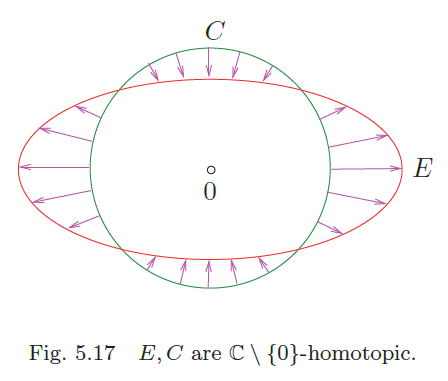
\includegraphics[width=0.4\textwidth]{./figs/fig-5-17}
\end{center}
\caption{$\mathbb C\setminus \{0\}$-호모토픽한 경로 $E$와 $C$}
\label{fig-5-17}
\end{figure}




 